
\begin{frame}
	\frametitle{Multidisciplinary Design Optimization (MDO)}
	\begin{itemize}
		\item Procedure that originated in the aerospace industry to systematically optimize complex engineering systems with cross discipline coupling
		\item WEC particularly well suited for MDO because strong disciplinary interdependencies (hydro, controls, powertrain, econ, structures)
		\item Compare to sequential design optimization
	\end{itemize}
	
\end{frame}


\begin{frame}
	\frametitle{Simulation Structure: XDSM Diagram}
	
	\centering
	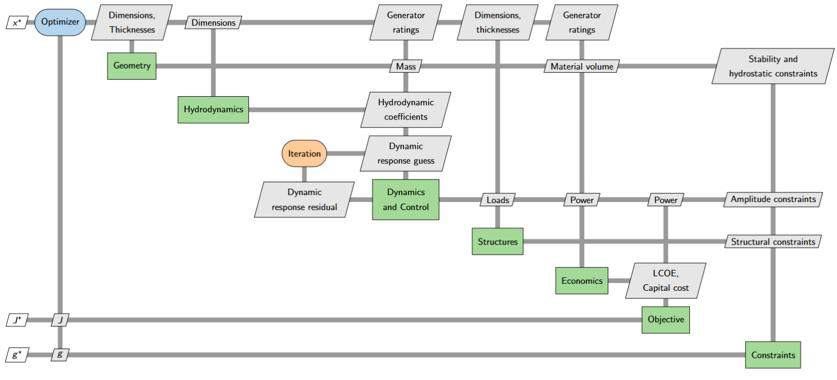
\includegraphics[width=\linewidth]{figs/img0002.png}
	
	{\footnotesize Runtime: 0.78 s}
	
\end{frame}


\begin{frame}
	\frametitle{Problem Formulation}
	\begin{itemize}
		\item Objective Function(s)
		      
		\item Inequality Constraint(s)
		      
		\item Equality Constraint(s)
		      
		\item Design
		\item Variable(s)
		      
		\item Upper
		\item Bound
		      
		\item Lower
		\item Bound
		      
		\item Parameter(s)
		      
		\item $h(x, p) =  0$
		      
		\item minimize $J(x, p)$
		      
		\item subject to $g(x, p) ＜ 0$
		      
		\item $x_{i,LB} \leq  x_i \leq  x_{i,UB}$
	\end{itemize}
	
\end{frame}


\begin{frame}
	\frametitle{Problem Formulation: J}
	\begin{tabular}{|l|l|} \hline
		Objective 1: LCOE                           & Objective 2: Pavg \\ \hline
		Levelized · Cost · of · Energy           & Average Power     \\ \hline
		$/kWh
		Electricity price over full system lifetime & kW                
		Annual mean power across all sea states  \\ \hline
	\end{tabular}
	
	
\end{frame}


\begin{frame}
	\frametitle{WEC Visuals}
	
	\centering
	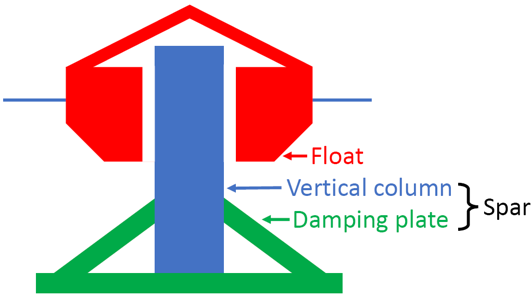
\includegraphics[width=0.9\linewidth]{figs/img0003.png}
	
\end{frame}


\begin{frame}
	\frametitle{WEC Visuals}
	
	\centering
	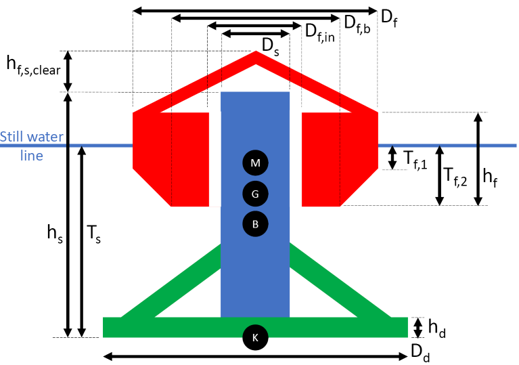
\includegraphics[width=0.9\linewidth]{figs/img0004.png}
	
\end{frame}


\begin{frame}
	\frametitle{Problem Formulation: x}
	
	\centering
	\begin{tabular}{|l|l|} \hline
		Design Variable & Description                    \\ \hline
		Df , Ds         & Diameter of float, spar        \\ \hline
		hfs,clear       & Height of float-spar clearance \\ \hline
		hs              & Height of spar                 \\ \hline
		Tf,2            & Draft of float                 \\ \hline
	\end{tabular}
	
	\begin{itemize}
		\item Geometry
		\item Control
	\end{itemize}
	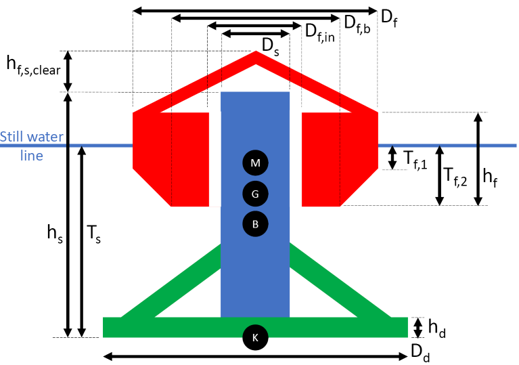
\includegraphics[width=0.9\linewidth]{figs/img0005.png}
	
\end{frame}


\begin{frame}
	\frametitle{Problem Formulation: x}
	
	\centering
	\begin{tabular}{|l|l|} \hline
		Design Variable       & Description                                                         \\ \hline
		Df , Ds               & Diameter of float, spar                                             \\ \hline
		hfs,clear             & Height of float-spar clearance                                      \\ \hline
		hs                    & Height of spar                                                      \\ \hline
		Tf,2                  & Draft of float                                                      \\ \hline
		Fmax, Pmax            & Maximum powertrain force, power                                     \\ \hline
		tf,b , ts,r , td      & Structural thickness of float (top), spar (radially), damping plate \\ \hline
		hstiff,f , h1,stiff,d & Stiffener height of float, damping plate                            \\ \hline
	\end{tabular}
	
	\begin{itemize}
		\item Geometry
		\item Control
	\end{itemize}
	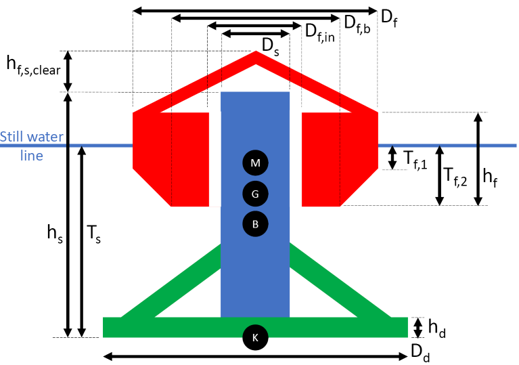
\includegraphics[width=0.9\linewidth]{figs/img0006.png}
	
\end{frame}


\begin{frame}
	\frametitle{Problem Formulation: p}
	\begin{itemize}
		\item 43 Parameters
		\item Dynamics
		\item Economics
		\item Structures
		\item Geometry
	\end{itemize}
	\begin{tabular}{|l|l|} \hline
		Parameter                  & Description                       \\ \hline
		Hs                         & Wave Height                       \\ \hline
		T                          & Wave Period                       \\ \hline
		ptoeff                     & Power Take-Off Efficiency         \\ \hline
		costm                      & Material Cost                     \\ \hline
		FCR                        & Fixed Charge Rate                 \\ \hline
		NWEC                       & # of WECs in Array                \\ \hline
		��y                    & Material Yield Strength           \\ \hline
		E                          & Material Young’s Modulus        \\ \hline
		⍴m                       & Material Density                  \\ \hline
		Dd/Ds                      & Normalized Damping Plate Diameter \\ \hline
		Ts/Ds                      & Normalized Spar Draft             \\ \hline
		Tf,2/hf                    & Normalized Float Draft            \\ \hline
		+ 31 Additional Parameters & + 31 Additional Parameters        \\ \hline
	\end{tabular}
	
	
\end{frame}


\begin{frame}
	\frametitle{Problem Formulation: g}
	
	\centering
	\begin{itemize}
		\item 233 Inequality Constraints
		      
		\item Factors of Safety (FOS) of 3 components to 2 load cases:
		\item Storm load to ultimate strength
		\item Operational load to fatigue strength
	\end{itemize}
	\begin{tabular}{|l|l|l|l|l|} \hline
		Constr.  & Description                          & <       & >      & Units \\ \hline
		hs,extra & Prevent  Float Above Top of the Spar & -       & 0      & m     \\ \hline
		Fp,max   & Obey Force Limit                     & Fmax    & Fmax   & N     \\ \hline
		Pp,max   & Obey Power Limit                     & Pmax    & -      & W     \\ \hline
		Xf/s,max & Obey Amplitude Limits                & Xmax    & -      & m     \\ \hline
		μ       & Net Generated Power                  & -       & 0      & kW    \\ \hline
		LCOE     & Prevent LCOE Greater Than Nominal    & LCOEmax & -      & $/kWh \\ \hline
		FOS      & Structural Factor of Safety          & -       & FOSmin & -     \\ \hline
		Vfpct    & Prevent Float too Heavy/Light        & 1       & 0      & -     \\ \hline
		Vspct    & Prevent Spar to Heavy/Light          & 1       & 0      & -     \\ \hline
		GM       & Metacentric Height                   & -       & 0      & m     \\ \hline
		Dd       & Minimum Damping Plate Diameter       & -       & Dd,min & m     \\ \hline
	\end{tabular}
	
	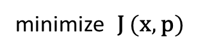
\includegraphics[width=0.9\linewidth]{figs/img0007.png}
	\begin{itemize}
		\item Dynamics
		\item Economics
		\item Structures
		\item Geometry
	\end{itemize}
	Float and spar hitting
	Float-spar overtravel
	Violating linear wave theory
	Float or spar slamming
	
\end{frame}

%%%%%%%%%%%%%%%%%%%%%%%%%%%%%%%%%%%%%%%%%%%%%%%%%%
\begin{frame}
	\frametitle{Agenda}
	\AgendaSlide{Results}
\end{frame}


\begin{frame}
	\frametitle{Optimization Pareto Front Results}
	
	\centering
	\begin{itemize}
		\item Pareto front of structures + PTO cost vs average power (with LCOE contours)
		\item Visualize effect of changing constant cost and fixed charge rate
		\item Power-maximizing control suboptimal for WECs $<60$~kW
		      
		\item McCabe, Dietrich, and Haji. “Leveraging Multidisciplinary Design Optimization to Advance Wave Energy Converter Viability.” In preparation for submission to Renewable Energy.
	\end{itemize}
	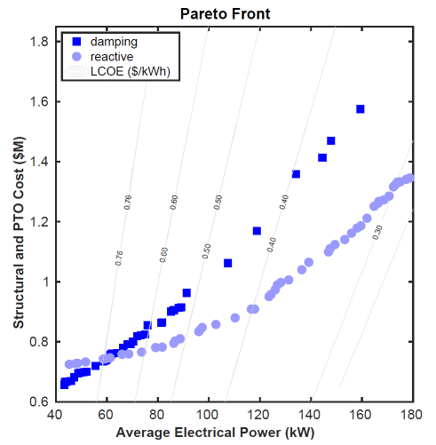
\includegraphics[width=0.4\linewidth]{figs/img0017.png}
	
\end{frame}


\begin{frame}
	\frametitle{Optimization Pareto Front Results}
	
	\centering
	\begin{itemize}
		\item Min LCOE design:
        \begin{itemize}
            \item 57\% lower LCOE
    		\item 37\% lower structural / powertrain cost
    		\item 89\% higher power 
        \end{itemize}
		\item McCabe, Dietrich, and Haji. “Leveraging Multidisciplinary Design Optimization to Advance Wave Energy Converter Viability.” In preparation for submission to Renewable Energy.
	\end{itemize}
	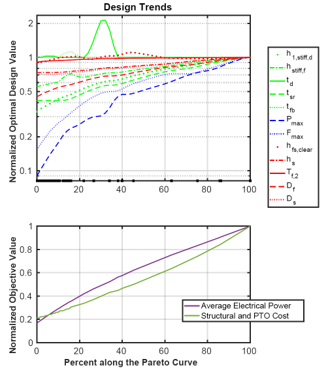
\includegraphics[width=0.4\linewidth]{figs/img0018.png}
	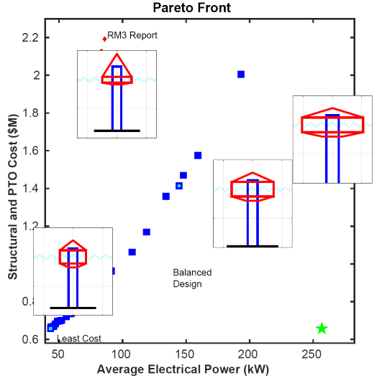
\includegraphics[width=0.4\linewidth]{figs/img0019.png}
	
\end{frame}


\begin{frame}
	\frametitle{Sensitivity Analysis to Address Economic Uncertainty}
	
	\centering
	\begin{itemize}
		\item Normalized: 1 means 10\% increase in parameter causes 10\% increase in objective
		\item $H_s$ and $T_{struct}$ (site wave conditions) are in top 10 for both objectives
		\item Most sensitive parameter is structural in both cases
	\end{itemize}
	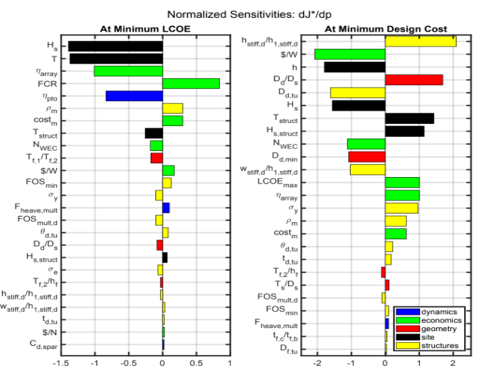
\includegraphics[width=0.8\linewidth]{figs/img0020.png}
	
	{\footnotesize McCabe, Dietrich, and Haji. “Leveraging Multidisciplinary Design Optimization to Advance Wave Energy Converter Viability.” In preparation for submission to Renewable Energy.}
	
\end{frame}


\begin{frame}
	\frametitle{Sensitivity Analysis to Address Economic Uncertainty}
	
	\centering
	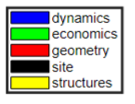
\includegraphics[width=0.1\linewidth]{figs/img0021.png}
	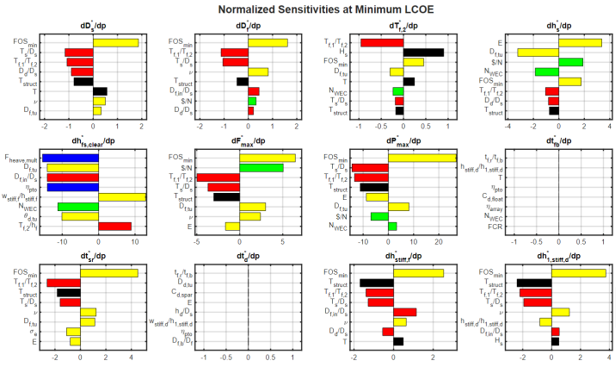
\includegraphics[width=0.9\linewidth]{figs/img0022.png}
	\begin{itemize}
		\item 7/12 are most sensitive to $FOS_{min}$
		\item $h_{fs,clear}$, $F_{max}$, and $P_{max}$ are highly sensitive
		      
		\item McCabe, Dietrich, and Haji. “Leveraging Multidisciplinary Design Optimization to Advance Wave Energy Converter Viability.” In preparation for submission to Renewable Energy.
		      
		\item $T_{f,1}$, $T_s$ possible future design variables
	\end{itemize}
	
\end{frame}


\begin{frame}
	\frametitle{Cost Optimization Takeaways}
	\begin{itemize}
		\item Multidisciplinary Design Optimization framework applied to bi-cylinder WEC
		\item Achieved 57\% lower LCOE and 89\% higher power
		\item Optimal pareto tradeoff curve
		\item Objectives have high sensitivity to sea states and economic parameters
		\item Optimal design has high sensitivity to geometric and structural parameters
	\end{itemize}
\end{frame}